\documentclass[main.tex]{subfiles}
\begin{document}
\section{Hypothèses}
\begin{itemize}
\item la non-linéarité est statique et n'évolue pas dans le temps. On peut la séparer de la dynamique du système. Par exemple, la saturation (ou la zone morte) est une non-linéarité statique.
\item la partie dynamique (linéaire) est un filtre passe-bas \emph{suffisamment efficace} pour négliger les harmoniques d'ordre supérieur à 1. Plus précisément, l'ordre relatif du filtre doit être supérieur strict à 1.
\end{itemize}

\section{Schéma-blocs}
\[ x \longrightarrow \boxed{
    \begin{array}{c}
      \text{Non} \\
      \text{Linéarité}
    \end{array}
} \longrightarrow y \longrightarrow \boxed{H(p)} \longrightarrow z \]
La fonction de transfert $H(p)$ (fraction rationnelle) correspond à un filtre passe-bas de degré relatif $\geq 2$.\\

On prend $x=X\sin \omega t$. Dans le cas linéaire, seule la valeur de $\omega$ influe sur le tracé de la diagramme de Bode du système. Dans le cas non-linéaire, on a plusieurs tracés de réponses fréquentielles. Par exemple, avec une saturation, on obtient des réponses fréquentielles qui dépendent de l'amplitude d'entrée de $X$ dès qu'elle devient trop élevée.

\begin{figure}[h!]
\centering
\begin{tikzpicture}
  \draw[-latex] (-4,0) -- (4,0)node[above]{$Re$};
  \draw[-latex] (0,-4) -- (0,4)node[left]{$Im$};
  \draw (0,0) to[out=110,in=0]  (-2,1)   to[out=180,in=80] (-4,-3) node[below]{$X_1$};
  \draw (0,0) to[out=130,in=0] (-1,0.7)  to[out=180,in=80] (-3,-3)node[below]{$X_2$};
  \draw (0,0) to[out=150,in=0] (-0.5,0.3) to[out=180,in=80](-2,-3) node[below]{$X_3$};
  \node[above] at (-2,1) {$T_{BO}$};
\end{tikzpicture}
 \caption{Modification du lieu en fonction de l'amplitude}
\end{figure}

Puisque $H(p)$ rejette les harmoniques d'ordre supérieur à 1, on peut donc décomposer \[y(t)=P \sin \omega t + Q \cos \omega t\]

Dans le cas d'une NL symétrique, on a
\begin{align*}
P& =\frac{2}{T} \int_{[T]} y(t) \sin \omega t dt\\
Q& =\frac{2}{T} \int_{[T]} y(t) \cos \omega t dt \quad \text{ avec } \omega T = 2\pi
\end{align*}

\begin{rem}
Si la NL est non-symétrique, $y(t) = Y+P\sin \omega t + Q \cos \omega t$ avec $Y=\frac{1}{T}\int_{[T]} y(t) dt$. La composante continue $Y$ peut être négligée pour l'analyse de stabilité et modélisée par une perturbation constante à l'entrée de $H(p)$.
\end{rem}
\begin{defin}
On définit le \emph{gain complexe équivalent}:
\[ N(X) = \frac{P+jQ}{X} \text{ qu'on note } N(X) = N_P(X) + jN_Q(X) \]
\begin{itemize}
\item $N_P(X)=\frac{P}{X}$ est la gain en phase,
\item $N_Q(X)=\frac{Q}{X}$ est la gain en quadrature.
\end{itemize}
\end{defin}

\begin{rem}
\begin{itemize}
\item À la différence du système linéaire, pour une même pulsation, on a plusieurs réponses fréquentielles qui dépendent de l'amplitude de l'entrée $X$. L'analyse de stabilité doit donc se faire par rapport à tous les tracés.

% Inclure le nyquist du génie

\item Les manipulations de schéma-blocs doivent satisfaire les règles connues (principe de superposition) et s'assurer que le signal en amont du bloc NL est le même, et en aval, qu'il est suffisamment filtré pour ne garer que le 1er harmonique.

\begin{example}
\begin{figure}[h!]
\centering
\begin{tikzpicture}
\sbEntree{E}

\sbComp[3]{comp}{E}
\sbRelier[$e$]{E}{comp}

\sbBloc[2]{C}{$C(p)$}{comp}
\sbRelier{comp}{C}

\sbBloc[2]{NL}{Non-linéarité}{C}
\sbRelier[$x$]{C}{NL}

\sbBloc[2]{sys}{$H(p)$}{NL}
\sbRelier{NL}{sys}

\sbSortie[2]{S}{sys}
\sbRelier{sys}{S}

\sbRenvoi{sys-S}{comp}{}

\end{tikzpicture}
\[
\Updownarrow
\]
\begin{tikzpicture}
\sbEntree{E}

\sbBloc[3]{C}{$C(p)$}{E}
\sbRelier[$e$]{E}{C}

\sbComp[4]{comp}{C}
\sbRelier{C}{comp}

\sbBloc[2]{NL}{Non-linéarité}{comp}
\sbRelier[$x$]{comp}{NL}

\sbBloc[2]{sys}{$H(p)$}{NL}
\sbRelier{NL}{sys}

\sbSortie[2]{S}{sys}
\sbRelier{sys}{S}

\sbDecaleNoeudy[4]{S}{R}
\sbBlocr[8]{Cr}{$C(p)$}{R}
\sbRelieryx{sys-S}{Cr}
\sbRelierxy{Cr}{comp}
\end{tikzpicture}
\[
 \Updownarrow\hspace{-0.8em}/
\]
\begin{tikzpicture}
\sbEntree{E}

\sbComp[3]{comp}{E}
\sbRelier[$e$]{E}{comp}

\sbBloc[4]{NL}{Non-linéarité}{comp}
\sbRelier[$\hat{x}\neq x$]{comp}{NL}

\sbBloc[2]{sys}{$H(p)C(p)$}{NL}
\sbRelier{NL}{sys}

\sbSortie[2]{S}{sys}
\sbRelier{sys}{S}

\sbRenvoi{sys-S}{comp}{}

\end{tikzpicture}
\caption{Transformations de schéma-blocs}
\end{figure}

\end{example}
\end{itemize}
\end{rem}

\newpage
\section{Analyse de la stabilité.}

Système NL bouclé à retour unitaire

\begin{figure}[h!]
\centering
\begin{tikzpicture}
\sbEntree{E}

\sbComp[4]{comp}{E}
\sbRelier[$e$]{E}{comp}

\sbBloc[4]{NL}{$N(X)$}{comp}
\sbRelier[$x$]{comp}{NL}

\sbBloc[4]{sys}{$T_{BO}(p)$}{NL}
\sbRelier{NL}{sys}

\sbSortie[4]{S}{sys}
\sbRelier{sys}{S}

\sbRenvoi{sys-S}{comp}{}

\end{tikzpicture}
\end{figure}

Dans l'analyse harmonique, la NL est modélisée par $N(X)$. Ainsi, il faut trouver l'expression de $N(X)$ en fonction de la NL :

\begin{exemple}[saturation]

\begin{figure}[h!]
  \centering
  \begin{tikzpicture}
    \begin{axis}
      [axis lines =middle,
      width=8cm, height=6cm,
      xlabel=$X$,ylabel=$Y$,
      xtick={-2,2},xticklabels={$-X_m$,$X_m$},
      ytick={-1.5,1.5},yticklabels={$-Y_m$,$Y_m$},
      ymin=-3,ymax=3, xmin=-5,xmax=5,
      ]
      \addplot[no marks,black] plot coordinates
      {(-4,-1.5) (-2,-1.5) (2,1.5) (4,1.5)};
      \addplot[no marks,dashed,black] plot coordinates
      {(-2,0) (-2,-1.5) (0,-1.5)};
      \addplot[no marks,dashed,black] plot coordinates
      {(2,0) (2,1.5) (0,1.5)};
    \end{axis}

    \begin{axis}[at ={(8cm,0cm)},
      width=10cm,height=6cm,
      axis lines =middle,
      xlabel=$t$,ylabel=$X$,
      xtick={1,2,3.1415},xticklabels={$t_1$,$\frac{\pi}{\omega}-t_1$,$\frac{\pi}{\omega}$},
      ytick={-2.1,2.1},yticklabels={$-X_m$,$X_m$},
      ymin=-3,ymax=3, xmin=0,xmax=7,
      domain=0:7,
      ]
      \addplot[no marks,black,smooth,dashed] {2.5*sin(deg(x))};
      \addplot[thick, no marks,domain=0:1]{2.5*sin(deg(x))};
      \addplot[thick, no marks,domain=2.1415:4.1415]{2.5*sin(deg(x))};
      \addplot[thick, no marks,domain=5.283:7]{2.5*sin(deg(x))};
      \addplot[thick, no marks] coordinates {(1,2.1) (2.1415,2.1)};
      \addplot[thick, no marks] coordinates {(4.1415,-2.1) (5.283,-2.1)};
    \end{axis}
  \end{tikzpicture}
\end{figure}

Calcul de $N(X)$ :

Pour $0 \leq t \leq t_1$ : $y(t) = X\sin \omega t$

$t_1 \leq t \leq \frac{\pi}{\omega}-t_1$ : $y(t) = X_m = X\sin \omega t_1$

\begin{align*}
P & = \frac{4\omega}{\pi} \int_0^{\frac{\pi}{2\omega}} y(t) \sin \omega t dt \\
& = \frac{4\omega}{\pi} [ \int_0^{t_1} X \sin^2 \omega t dt + \int_{t_1}^{\frac{\pi}{2\omega}} X \sin \omega t_1 \sin \omega t dt ] \\
& = \frac{2X}{\pi}[ \omega t_1 + \frac{\sin 2\omega t_1}{2} ] \\
\intertext{ $t_1=\arcsin(\frac{X_m}{X})$ et $Q=0$}
\intertext{Ainsi}
N(x) & =
       \begin{cases}
         1 & \si X << X_m\\
         \frac{2}{\pi}[\arcsin\frac{X_m}{X}+\frac{X_m}{X}\sqrt{1-\frac{X_m^2}{X^2}}] & \si X > X_m
       \end{cases}
\end{align*}
\begin{prop}
  Le dénominateur de la BF, $1+N(X)T_{BO}(p)$, donne la limite de stabilité : \[T_{BO}(j\omega) = - \frac{1}{N(X)}\]

  Le lieu critique remplace le point critique $-1$.
\end{prop}
On a donc pour notre exemple de saturation

\begin{figure}[h!]
  \centering
  \begin{tikzpicture}
    \begin{axis}
      [axis lines= middle,
      xmin=-4,xmax=3,ymin=-2,ymax=3,ticks=none,
      xlabel=$Re$,ylabel=$Im$]
      \addplot[smooth,tension=1,-latex] coordinates {(-2.5,-3) (-2,0) (-1,1.5)};
      \addplot[smooth,tension=1]coordinates{ (-1,1.5) (-0.3,1.2) (0,0)};
      \addplot[smooth,thick,|-latex] coordinates {(-2.5,0) (-4,0)};
       \node[above] at (axis cs:-1,1.5) {$T_{BO}(j\omega)$};
      \node[below] at (axis cs: -3,0) {$-\frac{1}{N(X)}$};
    \end{axis}
  \end{tikzpicture}
  \caption{INSTABLE} 
\end{figure}

\end{exemple}

Ainsi dans le cas NL, on remplace le point critique $-1$ par le lieu critique $\frac{-1}{N(X)}$. Par conséquent, l'analyse de stabilité est réalisée par rapport à $\frac{-1}{N(X)}$.
On a alors deux cas
\begin{enumerate}
\item
  Dans le cas où le tracé de Nyquist ne présente \emph{pas d'intersection avec le lieu critique}

  on applique le critère de Nyquist ($ N_{\frac{1}{N(Y)}^{+}} = P^T_{T_{BO}}$) pour la stabilité ou celui du revers sur la FT, qui est alors stable, strictement propre et à déphasage minimal.

\item Si on a une ou plusieurs intersections, on a un régime auto-oscillant (cycle limite). $x(t) = X_0 e^{j\omega_0 t}$
\end{enumerate}
\section{Étude de la stabilité du cycle limite}

Soit $(X_0,\omega_0)$ solution de $T_{B0}(j\omega_0)=-\frac{1}{N(X_0)}$ sur son cycle limite :
\[
  x(t)= X_0e^{j\omega_0t}
\]

\subsection{Critère analytique}

On pose \[T_{B0}(j\omega)+\frac{1}{N(X_0)}=R(\omega,X)+jI(\omega,X) = 0\]

Ainsi, on a \[R(\omega_0,X_0)=0 \text{ et }I(\omega_0,X_0)=0\]
Pour analyser la stabilité on applique À $t_0$  une perturbation :
\[X_1 = X_0 + \delta X \text{ et }\omega_1 = \omega_0+\delta \omega \quad \text{ avec } |\frac{\delta X}{X_0}|<<1 \text{ et }|\frac{\delta \omega}{\omega_0}|<<1 \]

$x(t)$ n'est plus périodique (plus d'intersection avec le lieu critique) et présente ainsi un amortissement $m>0$ (stable) ou $<0$ (instable).

\[ x(t) = (X_0 + \delta X) e^{-mt} e^{j(\omega_0 + \delta \omega) t} =(X_0 + \delta X) e^{j(\omega_0 + \delta \omega + jm) t} \]

Ainsi la perturbation nous donne un régime auto-oscillant avec une amplitude $X_0+\delta X$ et une \emph{pulsation complexe} $\omega_0 + \delta \omega + jm$.

\[ R(\omega_0+\delta \omega + jm, X_0 + \delta X) + jI(\omega_0 + \delta \omega + jm,X_0 + \delta X) = 0 \]

\newcommand{\zero}{(\omega_0,X_0)}
On applique un DL du 1er ordre autour de $\zero$ :
\[ \left(\left.\derivp[R]{X}\right|_{\zero} + j \left.\derivp[I]{X}\right|_{\zero}\right) \delta X + \left(\left.\derivp[R]{\omega}\right|_{\zero} + j \left.\derivp[I]{\omega}\right|_{\zero}\right)(\delta \omega + jm)\approx 0 \]
i.e. en notant $\left.\derivp[]{X}\right|_{\zero}=\left.\derivp[]{X}\right|_0$
\begin{align*}
\derivp[R]{\omega}|_0 .\delta \omega + \derivp[R]{X}|_0 .\delta X - \derivp[I]{\omega}|_0 .m & = 0 \\
\text{ et }\quad \derivp[I]{\omega}|_0 .\delta \omega + \derivp[I]{X}|_0 .\delta X + \derivp[R]{\omega}|_0 .m & = 0
\end{align*}

Élimination de $\delta \omega$ :
\[\underbracket{ \left( \left(\left.\derivp[R]{\omega}\right|_0\right)^2 + \left(\left.\derivp[I]{\omega}\right|_0\right)^2 \right)}_{\ge 0} m
  = \left( \left.\derivp[R]{X}\right|_0.\left.\derivp[I]{\omega}\right|_0 - \left.\derivp[R]{\omega}\right|_0.\left.\derivp[I]{X}\right|_0 \right) \delta X \]

\newpage
\noindent Différents types de perturbation

\begin{figure}[h!]
  \centering
  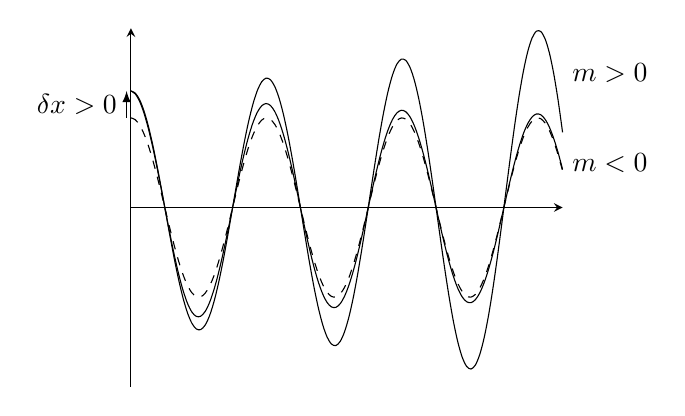
\begin{tikzpicture}
    \begin{axis}
      [axis lines= middle,scale=0.8,
      ticks=none, domain=0:10,samples=100,
      xmin=0,xmax=10,ymin=-2,ymax=2,clip=false]
      \addplot[black,smooth,dashed]{cos(2*deg(x))};
      \addplot[black,smooth]{cos(2*deg(x))*(1+0.3*exp(x/8))};
      \addplot[black,smooth]{cos(2*deg(x))*(1+0.3*exp(-x/5))};
      \draw[-latex] (axis cs: -0.1,1) -- (axis cs: -0.1,1.3) node[midway,left]{$\delta x >0 $};
      \draw (axis cs:10,1.5) node[right]{$m>0$};
      \draw (axis cs:10,0.5) node[right]{$m<0$};
    \end{axis}
  \end{tikzpicture}\qquad%
  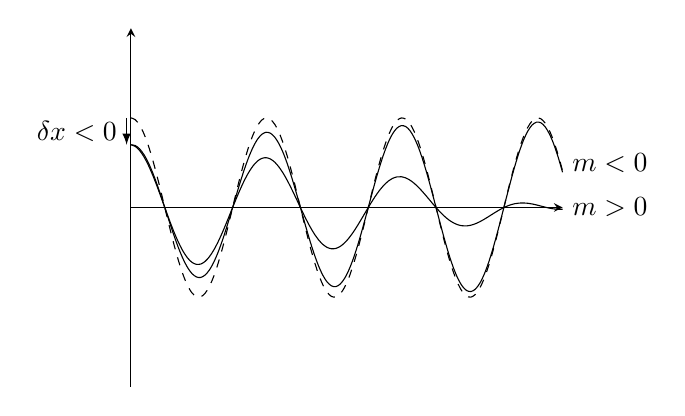
\begin{tikzpicture}
  \begin{axis}
      [axis lines= middle,scale=0.8,
      ticks=none, domain=0:10,samples=100,
      xmin=0,xmax=10,ymin=-2,ymax=2,clip=false]
      \addplot[black,smooth,dashed]{cos(2*deg(x))};
      \addplot[black,smooth]{cos(2*deg(x))*(1-0.3*exp(x/8))};
      \addplot[black,smooth]{cos(2*deg(x))*(1-0.3*exp(-x/5))};
      \draw[-latex] (axis cs: -0.1,1) -- (axis cs: -0.1,0.7) node[midway,left]{$\delta x< 0$};
      \draw (axis cs:10,0) node[right]{$m>0$};
      \draw (axis cs:10,0.5) node[right]{$m<0$};
    \end{axis}
  
  \end{tikzpicture}
\end{figure}
$m > 0$ et $\delta X > 0$ : CL est stable

$m < 0$ et $\delta X > 0$ : CL est instable

$\delta X < 0$ et $m < 0$ : CL est stable

$\delta X < 0$ et $m > 0$ : CL est instable

\begin{prop}[Condition de stabilité du cycle limite dans le plan de Nyquist]
le cycle limite est stable si et seulement si $\delta X . m >0$\\

Pour que $\delta X . m >0$ :
\[\boxed{ \left.\derivp[R]{X}\right|_0.\left.\derivp[I]{\omega}\right|_0 - \left.\derivp[R]{\omega}\right|_0.\left.\derivp[I]{X}\right|_0 > 0 }\]
\end{prop}

On pose $T_{B0}(j\omega) = U(\omega) + jV(\omega)$ et $-\frac{1}{N(X)} = L(X) + jM(X)$

On a un cycle limite si
\[ T_{B0}(j\omega_0) = -\frac{1}{N(x)} \quad \Rightarrow \quad
  \begin{cases}
R(\omega,X) & = U(\omega) - L(X)\\I(\omega,X) & = V(\omega) - M(X)
\end{cases}
\]

d'où d'après la condition de stabilité du cycle limite :
\[\boxed{-\derivp[L]{X}|_0.\derivp[V]{\omega}|_0 + \derivp[U]{\omega}|_0.\derivp[M]{X}|_0 > 0}\]

\subsection{Critère graphique}
On repart de l'équation caractéristique du cycle limite:
\[
  T_{BO}(j\omega) + \frac{1}{N(X)} = 0
\]
On note alors :
\[
  \begin{cases}
    T_{BO}(j\omega) = U(\omega)+j V(\omega) \\
    -\frac{1}{N(X)} = P(X)+j Q(X) \\
  \end{cases}
  \implies
  \begin{cases}
    \Re(X,\omega) = U(\omega)-P(X)\\
    \Im{X,\omega} = V(\omega)-Q(X)
  \end{cases}
\]

La condition de stabilité du cycle limite devient :
\[
  \left.\derivp[Q]{X}\right|_0 \left.\derivp[U]{\omega}\right|_0 - \left.\derivp[V]{\omega}\right|_0 \left.\derivp[P]{X}\right|_0 >0
\]
Si on se place dans $\R^3$, on a 2 vecteurs : $\vect{U\\V\\0}$ et $\vect{P\\Q\\0}$ qui décrivent respectivement $T_{BO}$ et $-\frac{1}{N}$.

Les tangentes aux courbes $T_{BO}$ et $-\frac{1}{N}$ sont colinéaires aux vecteurs:
\[\vec{v_T} = \derivp[]{\omega}\vect{U\\V\\0} \text{ et } \vec{u_N}=\derivp[]{X}\vect{P\\Q\\0} \text{ alors }
\vec{v_T}\wedge\vec{u_N} = \vect{0\\0\\-\derivp[P]{X}.\derivp[V]{\omega} + \derivp[U]{\omega}.\derivp[Q]{X}}\]

Ainsi, la condition $-\derivp[P]{X}.\derivp[V]{\omega} + \derivp[U]{\omega}.\derivp[Q]{X}>0 \Rightarrow (\vec{v_T},\vec{u_N})$ dans le sens direct.

\begin{figure}[h!]
  \centering
  \begin{subfigure}{.5\textwidth}
    \centering
    \begin{tikzpicture}
    \begin{axis}
      [axis lines= middle,name=plot1,
      at={(0,0)},
      xmin=-3,xmax=3,ymin=-3,ymax=3,ticks=none,
      xlabel=$Re$,ylabel=$Im$]
      \addplot[smooth,tension=1,-latex] coordinates {(-2.5,-3) (-2,0) (-1,1.5)};
      \addplot[smooth,tension=1]coordinates{ (-1,1.5) (-0.3,1.2) (0,0)};
      \addplot[smooth,tension=1,-latex] coordinates {(0,-4) (-1,-2) (-3,-1)};
      \node[above] at (axis cs:-1,1.5) {$T_{BO}(j\omega)$};
      \node[above] at (axis cs: -1,-2) {$-\frac{1}{N(X)}$};
    \end{axis}
  \end{tikzpicture}
  \caption{STABLE}
\end{subfigure}%
\begin{subfigure}{.5\textwidth}
  \centering
  \begin{tikzpicture}
    \begin{axis}
      [axis lines= middle,
      xmin=-3,xmax=3,ymin=-3,ymax=3,ticks=none,
      xlabel=$Re$,ylabel=$Im$]
      \addplot[smooth,tension=1,-latex] coordinates {(-2.5,-3) (-2,0) (-1,1.5)};
      \addplot[smooth,tension=1]coordinates{ (-1,1.5) (-0.3,1.2) (0,0)};
      \addplot[smooth,tension=1,-latex] coordinates {(-3,-2) (-2,-1) (-0.5,-0.5)};
       \node[above] at (axis cs:-1,1.5) {$T_{BO}(j\omega)$};
      \node[below] at (axis cs: -1,-1) {$-\frac{1}{N(X)}$};
    \end{axis}
  \end{tikzpicture}
  \caption{INSTABLE}
\end{subfigure}
\caption{Critère géométrique de stabilité}
\end{figure}

\begin{thm}[Critère de Loeb]
Le cycle limite est stable si l'intersection de $T_{BO}(j\omega)$ et de $-\frac{1}{N(X)}$ est telle qu'en parcourant le lieu de Nyquist $T_{BO}(j\omega)$ dans le sens des $\omega$ croissants, on laisse à gauche la direction des $X$ croissant sur le lieu critique.
\end{thm}
\end{document}

%%% Local Variables:
%%% mode: latex
%%% TeX-master: "main"
%%% End:
